\section{Experiments}
\label{supp:sec:experiments}
\subsection{Experimental Setup}
\label{supp:sec:experimental_setup}
Our simulation environment is built upon MineDojo~\cite{fan2022minedojo} and utilizes Mineflayer~\cite{mineflayer} JavaScript APIs for motor controls (Sec.~\ref{supp:sec:skill_library_prompt}). Additionally, we incorporate many \texttt{bot.chat()} into Mineflayer functions to provide abundant environment feedback and implement various condition checks along with try-catch exceptions for continuous execution. If the bot dies, it is resurrected near the closest ground, and its inventory is preserved for uninterrupted exploration. The bot recycles its crafting table and furnace after program execution. For detailed implementations, please refer to our codebase.

\subsection{Baselines}
\textbf{ReAct}~\cite{yao2022react} uses chain-of-thought prompting~\cite{wei2022chain} by generating both reasoning traces and action plans with LLMs. We provide it with our environment feedback and the agent states as observations. ReAct undergoes one round of code generation from scratch, followed by three rounds of code refinement. This process is then repeated until the maximum prompting iteration is reached.

\textbf{Reflexion}~\cite{shinn2023reflexion} is built on top of ReAct~\cite{yao2022react} with self-reflection to infer more intuitive future actions. We provide it with environment feedback, the agent states, execution errors, and our self-verification module. Similar to ReAct, Reflexion undergoes one round of code generation from scratch, followed by three rounds of code refinement. This process is then repeated until the maximum prompting iteration is reached.

\textbf{AutoGPT}~\cite{autogpt} is a popular software tool that automates NLP tasks by decomposing a high-level goal into multiple subgoals and executing them in a ReAct-style loop. We re-implement AutoGPT by using GPT-4 to do task decomposition and provide it with the agent states, environment feedback, and execution errors as observations for subgoal execution. Compared with \voyager, AutoGPT lacks the skill library for accumulating knowledge, self-verification for assessing task success, and automatic curriculum for open-ended exploration. During each subgoal execution, if no execution error occurs, we consider the subgoal completed and proceed to the next one. Otherwise, we refine the program until three rounds of code refinement (equivalent to four rounds of code generation) are completed, and then move on to the next subgoal. If three consecutive subgoals do not result in acquiring a new item, we replan by rerunning the task decomposition.

The task is ``explore the world and get as many items as possible'' for all baselines.

\begin{table}[!ht]
\vskip 0.1in
\centering
\caption{Comparison between \voyager and baselines.}
\resizebox{\textwidth}{!}{
    \begin{tabular}{l|cccc}
    \toprule
    & ReAct~\cite{yao2022react} & Reflexion~\cite{shinn2023reflexion} & AutoGPT~\cite{autogpt} & \voyager \\
    \midrule
    Chain-of-Thought~\cite{wei2022chain} & $\checkmark$ & $\checkmark$ & $\checkmark$ & $\checkmark$ \\
    Self Verification & & $\checkmark$ & & $\checkmark$ \\
    Environment Feedback & $\checkmark$ & $\checkmark$ & $\checkmark$ & $\checkmark$ \\
    Execution Errors & & $\checkmark$ & $\checkmark$ & $\checkmark$ \\
    Agent State & $\checkmark$ & $\checkmark$ & $\checkmark$ & $\checkmark$ \\
    Skill Library & & & & $\checkmark$ \\
    Automatic Curriculum & & & & $\checkmark$ \\
    \bottomrule
    \end{tabular}
}
% \vspace{-1em}
% \vskip -0.1in
\label{supp:table:baseline_comparison}
\end{table}

\subsection{Ablations}
\label{supp:sec:ablations}
We ablate 6 design choices (automatic curriculum, skill library, environment feedback, execution errors, self-verification, and GPT-4 for code generation) in \voyager and study their impact on exploration performance.
\begin{itemize}
    \item \textbf{Manual Curriculum}: We substitute the automatic curriculum with a manually designed curriculum for mining a diamond: ``Mine 3 wood log'', ``Craft 1 crafting table'', ``Craft 1 wooden pickaxe'', ``Mine 11 cobblestone'', ``Craft 1 stone pickaxe'', ``Craft 1 furnace'', ``Mine 3 iron ore'', ``Smelt 3 iron ore'', ``Craft 1 iron pickaxe'', ``Mine 1 diamond''. A manual curriculum requires human effort to design and is not scalable for open-ended exploration.
    \item \textbf{Random Curriculum}: We curate 101 items obtained by \voyager and create a random curriculum by randomly selecting one item as the next task.
    \item \textbf{w/o Skill Library}: We remove the skill library, eliminating skill retrieval for code generation.
    \item \textbf{w/o Environment Feedback}: We exclude environment feedback (chat log) from the prompt for code generation.
    \item \textbf{w/o Execution Errors}: We exclude execution errors from the prompt for code generation.
    \item \textbf{w/o Self-Verification}: For each task, we generate code without self-verification and iteratively refine the program for 3 rounds (equivalent to 4 rounds of code generation in total).
    \item \textbf{GPT-3.5}: We replace GPT-4 with GPT-3.5 for code generation. We retain GPT-4 for the automatic curriculum and the self-verification module.
\end{itemize}

\subsection{Evaluation Results}
\subsubsection{Significantly Better Exploration}
\begin{figure}[t]
    \centering
    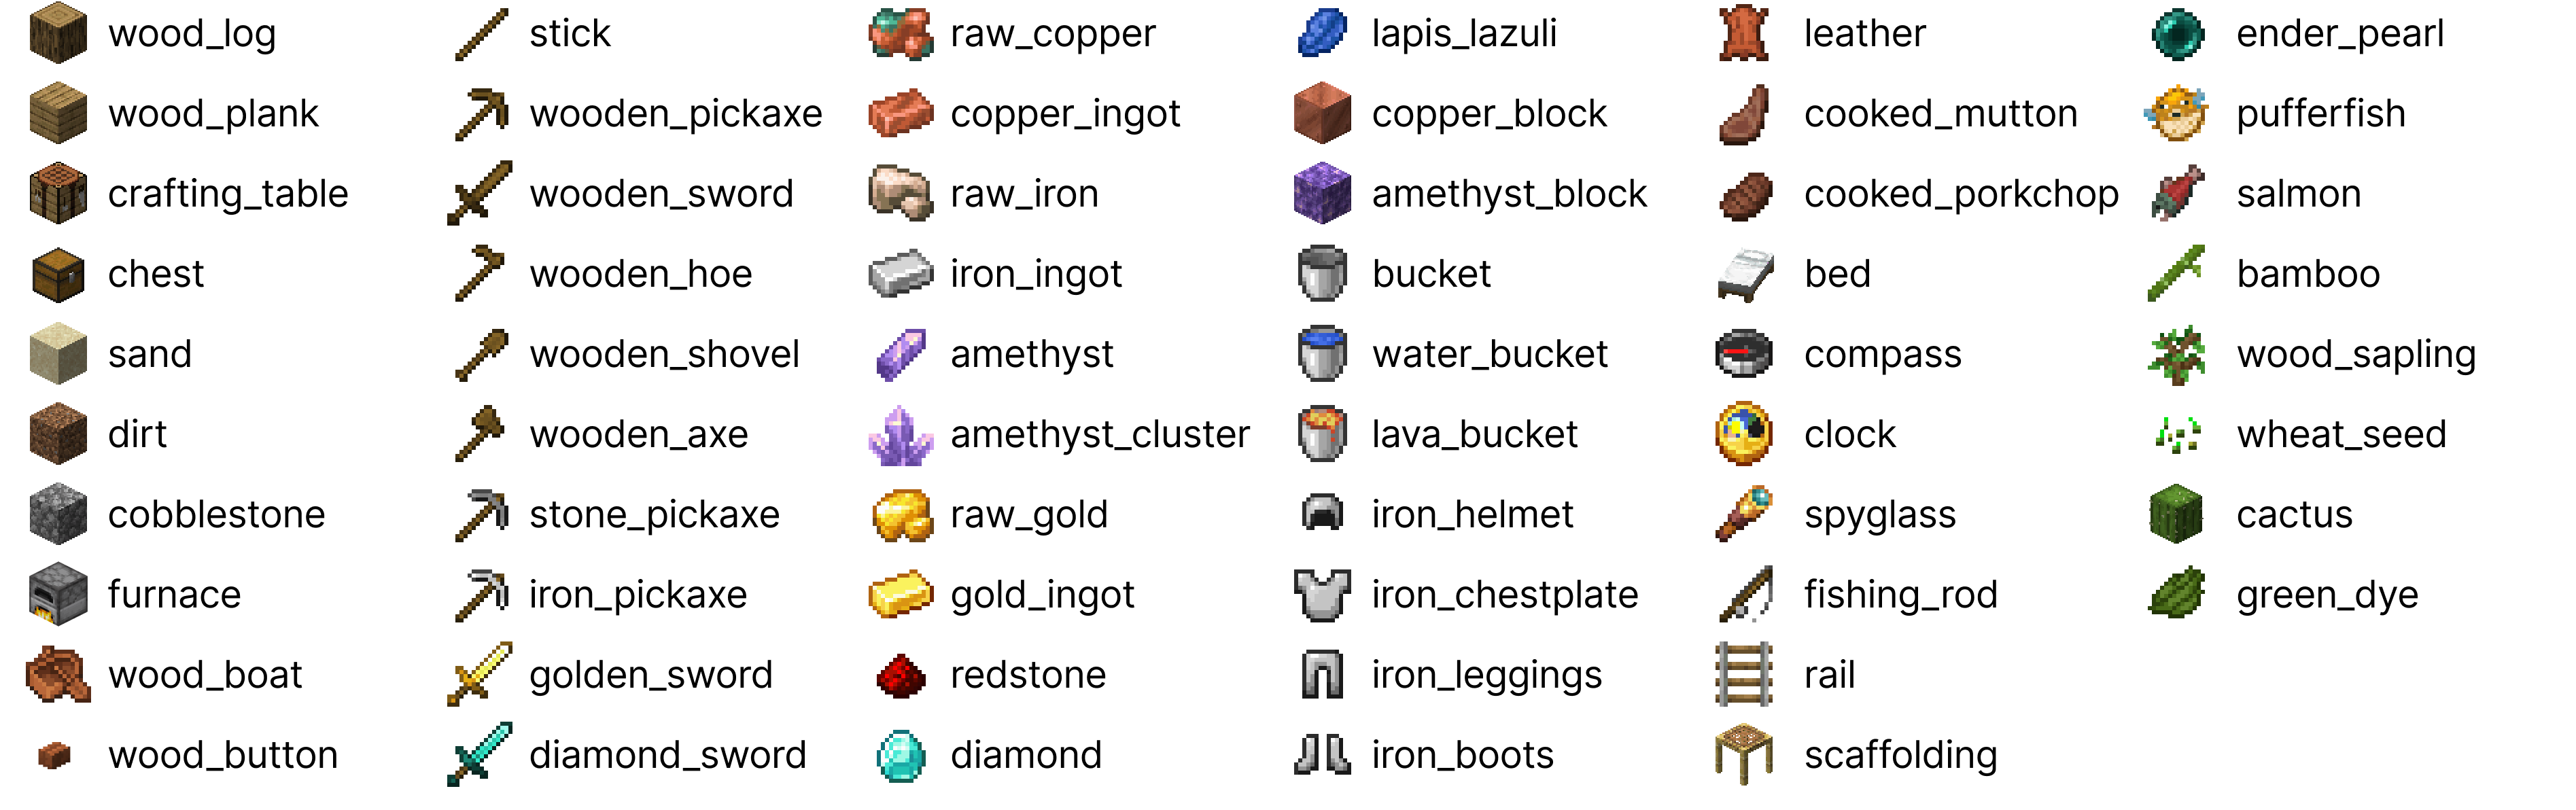
\includegraphics[width=\textwidth]{appendix/figures/mc_icons_fig.png}
    \vspace{0.05em}
    \caption{Minecraft item icons with corresponding names.}
    \label{supp:fig:icons}
    \vspace{-1em}
\end{figure}
The meaning of each icon in Fig.~\ref{fig:main_experiment} is shown in Fig.~\ref{supp:fig:icons}.

We run three trials for each method. The items collected by \voyager in each trial is \begin{itemize}
    \item \textbf{Trial 1}: {`iron\_ingot', `stone\_shovel', `iron\_leggings', `fishing\_rod', `pufferfish', `oak\_log', `cooked\_mutton', `green\_dye', `flint', `chest', `iron\_sword', `string', `ender\_pearl', `raw\_copper', `crafting\_table', `cactus', `lapis\_lazuli', `iron\_pickaxe', `copper\_ingot', `stone\_pickaxe', `wooden\_hoe', `scaffolding', `stick', `porkchop', `copper\_block', `gravel', `grass\_block', `white\_bed', `bone', `dirt', `mutton', `white\_wool', `oak\_sapling', `coal', `bamboo', `wooden\_pickaxe', `rotten\_flesh', `cooked\_porkchop', `cod', `iron\_boots', `lightning\_rod', `diorite', `water\_bucket', `shears', `furnace', `andesite', `granite', `bucket', `wooden\_sword', `sandstone', `iron\_helmet', `raw\_iron', `sand', `acacia\_log', `cooked\_cod', `oak\_planks', `azure\_bluet', `iron\_shovel', `acacia\_planks', `shield', `iron\_axe', `iron\_chestplate', `cobblestone'};
    \item \textbf{Trial 2}: {`iron\_ingot', `tuff', `stone\_shovel', `iron\_leggings', `fishing\_rod', `cooked\_mutton', `spruce\_planks', `gunpowder', `amethyst\_shard', `chest', `string', `cooked\_salmon', `iron\_sword', `raw\_copper', `crafting\_table', `torch', `lapis\_lazuli', `iron\_pickaxe', `copper\_ingot', `stone\_pickaxe', `wooden\_hoe', `stick', `amethyst\_block', `salmon', `calcite', `gravel', `white\_bed', `bone', `dirt', `mutton', `white\_wool', `spyglass', `coal', `wooden\_pickaxe', `cod', `iron\_boots', `lily\_pad', `cobbled\_deepslate', `lightning\_rod', `snowball', `stone\_axe', `smooth\_basalt', `diorite', `water\_bucket', `furnace', `andesite', `bucket', `granite', `shield', `iron\_helmet', `raw\_iron', `cobblestone', `spruce\_log', `cooked\_cod', `tripwire\_hook', `stone\_hoe', `iron\_chestplate', `stone\_sword'};
    \item \textbf{Trial 3}: {`spruce\_planks', `dirt', `shield', `redstone', `clock', `diamond\_sword', `iron\_chestplate', `stone\_pickaxe', `leather', `string', `chicken', `chest', `diorite', `iron\_leggings', `black\_wool', `cobblestone\_wall', `cobblestone', `cooked\_chicken', `feather', `stone\_sword', `raw\_gold', `gravel', `birch\_planks', `coal', `cobbled\_deepslate', `oak\_planks', `iron\_pickaxe', `granite', `tuff', `crafting\_table', `iron\_helmet', `stone\_hoe', `iron\_ingot', `stone\_axe', `birch\_boat', `stick', `sand', `bone', `raw\_iron', `beef', `rail', `oak\_sapling', `kelp', `gold\_ingot', `birch\_log', `wheat\_seeds', `cooked\_mutton', `furnace', `arrow', `stone\_shovel', `white\_wool', `andesite', `jungle\_slab', `mutton', `iron\_sword', `copper\_ingot', `diamond', `torch', `oak\_log', `cooked\_beef', `copper\_block', `flint', `bone\_meal', `raw\_copper', `wooden\_pickaxe', `iron\_boots', `wooden\_sword'}.
\end{itemize}
The items collected by ReAct~\cite{yao2022react} in each trial is \begin{itemize}
    \item \textbf{Trial 1}: {`bamboo', `dirt', `sand', `wheat\_seeds'};
    \item \textbf{Trial 2}: {`dirt', `rabbit', `spruce\_log', `spruce\_sapling'};
    \item \textbf{Trial 3}: {`dirt', `pointed\_dripstone'};
\end{itemize}
The items collected by Reflexion~\cite{shinn2023reflexion} in each trial is \begin{itemize}
    \item \textbf{Trial 1}: {`crafting\_table', `orange\_tulip', `oak\_planks', `oak\_log', `dirt'};
    \item \textbf{Trial 2}: {`spruce\_log', `dirt', `clay\_ball', `sand', `gravel'};
    \item \textbf{Trial 3}: {`wheat\_seeds', `oak\_log', `dirt', `birch\_log', `sand'}.
\end{itemize}
The items collected by AutoGPT~\cite{autogpt} in each trial is \begin{itemize}
    \item \textbf{Trial 1}: {`feather', `oak\_log', `leather', `stick', `porkchop', `chicken', `crafting\_table', `wheat\_seeds', `oak\_planks', `dirt', `mutton'};
    \item \textbf{Trial 2}: {`wooden\_pickaxe', `iron\_ingot', `stone', `coal', `spruce\_planks', `string', `raw\_copper', `crafting\_table', `diorite', `andesite', `furnace', `torch', `spruce\_sapling', `granite', `iron\_pickaxe', `stone\_pickaxe', `wooden\_axe', `raw\_iron', `stick', `spruce\_log', `dirt', `cobblestone'};
    \item \textbf{Trial 3}: {`wooden\_shovel', `wooden\_pickaxe', `iron\_ingot', `stone', `cod', `coal', `oak\_log', `flint', `raw\_copper', `crafting\_table', `diorite', `furnace', `andesite', `torch', `granite', `lapis\_lazuli', `iron\_pickaxe', `stone\_pickaxe', `raw\_iron', `stick', `gravel', `oak\_planks', `dirt', `iron\_axe', `cobblestone'}.
\end{itemize}

\subsubsection{Extensive Map Traversal}
\begin{figure}[t]
    \centering
    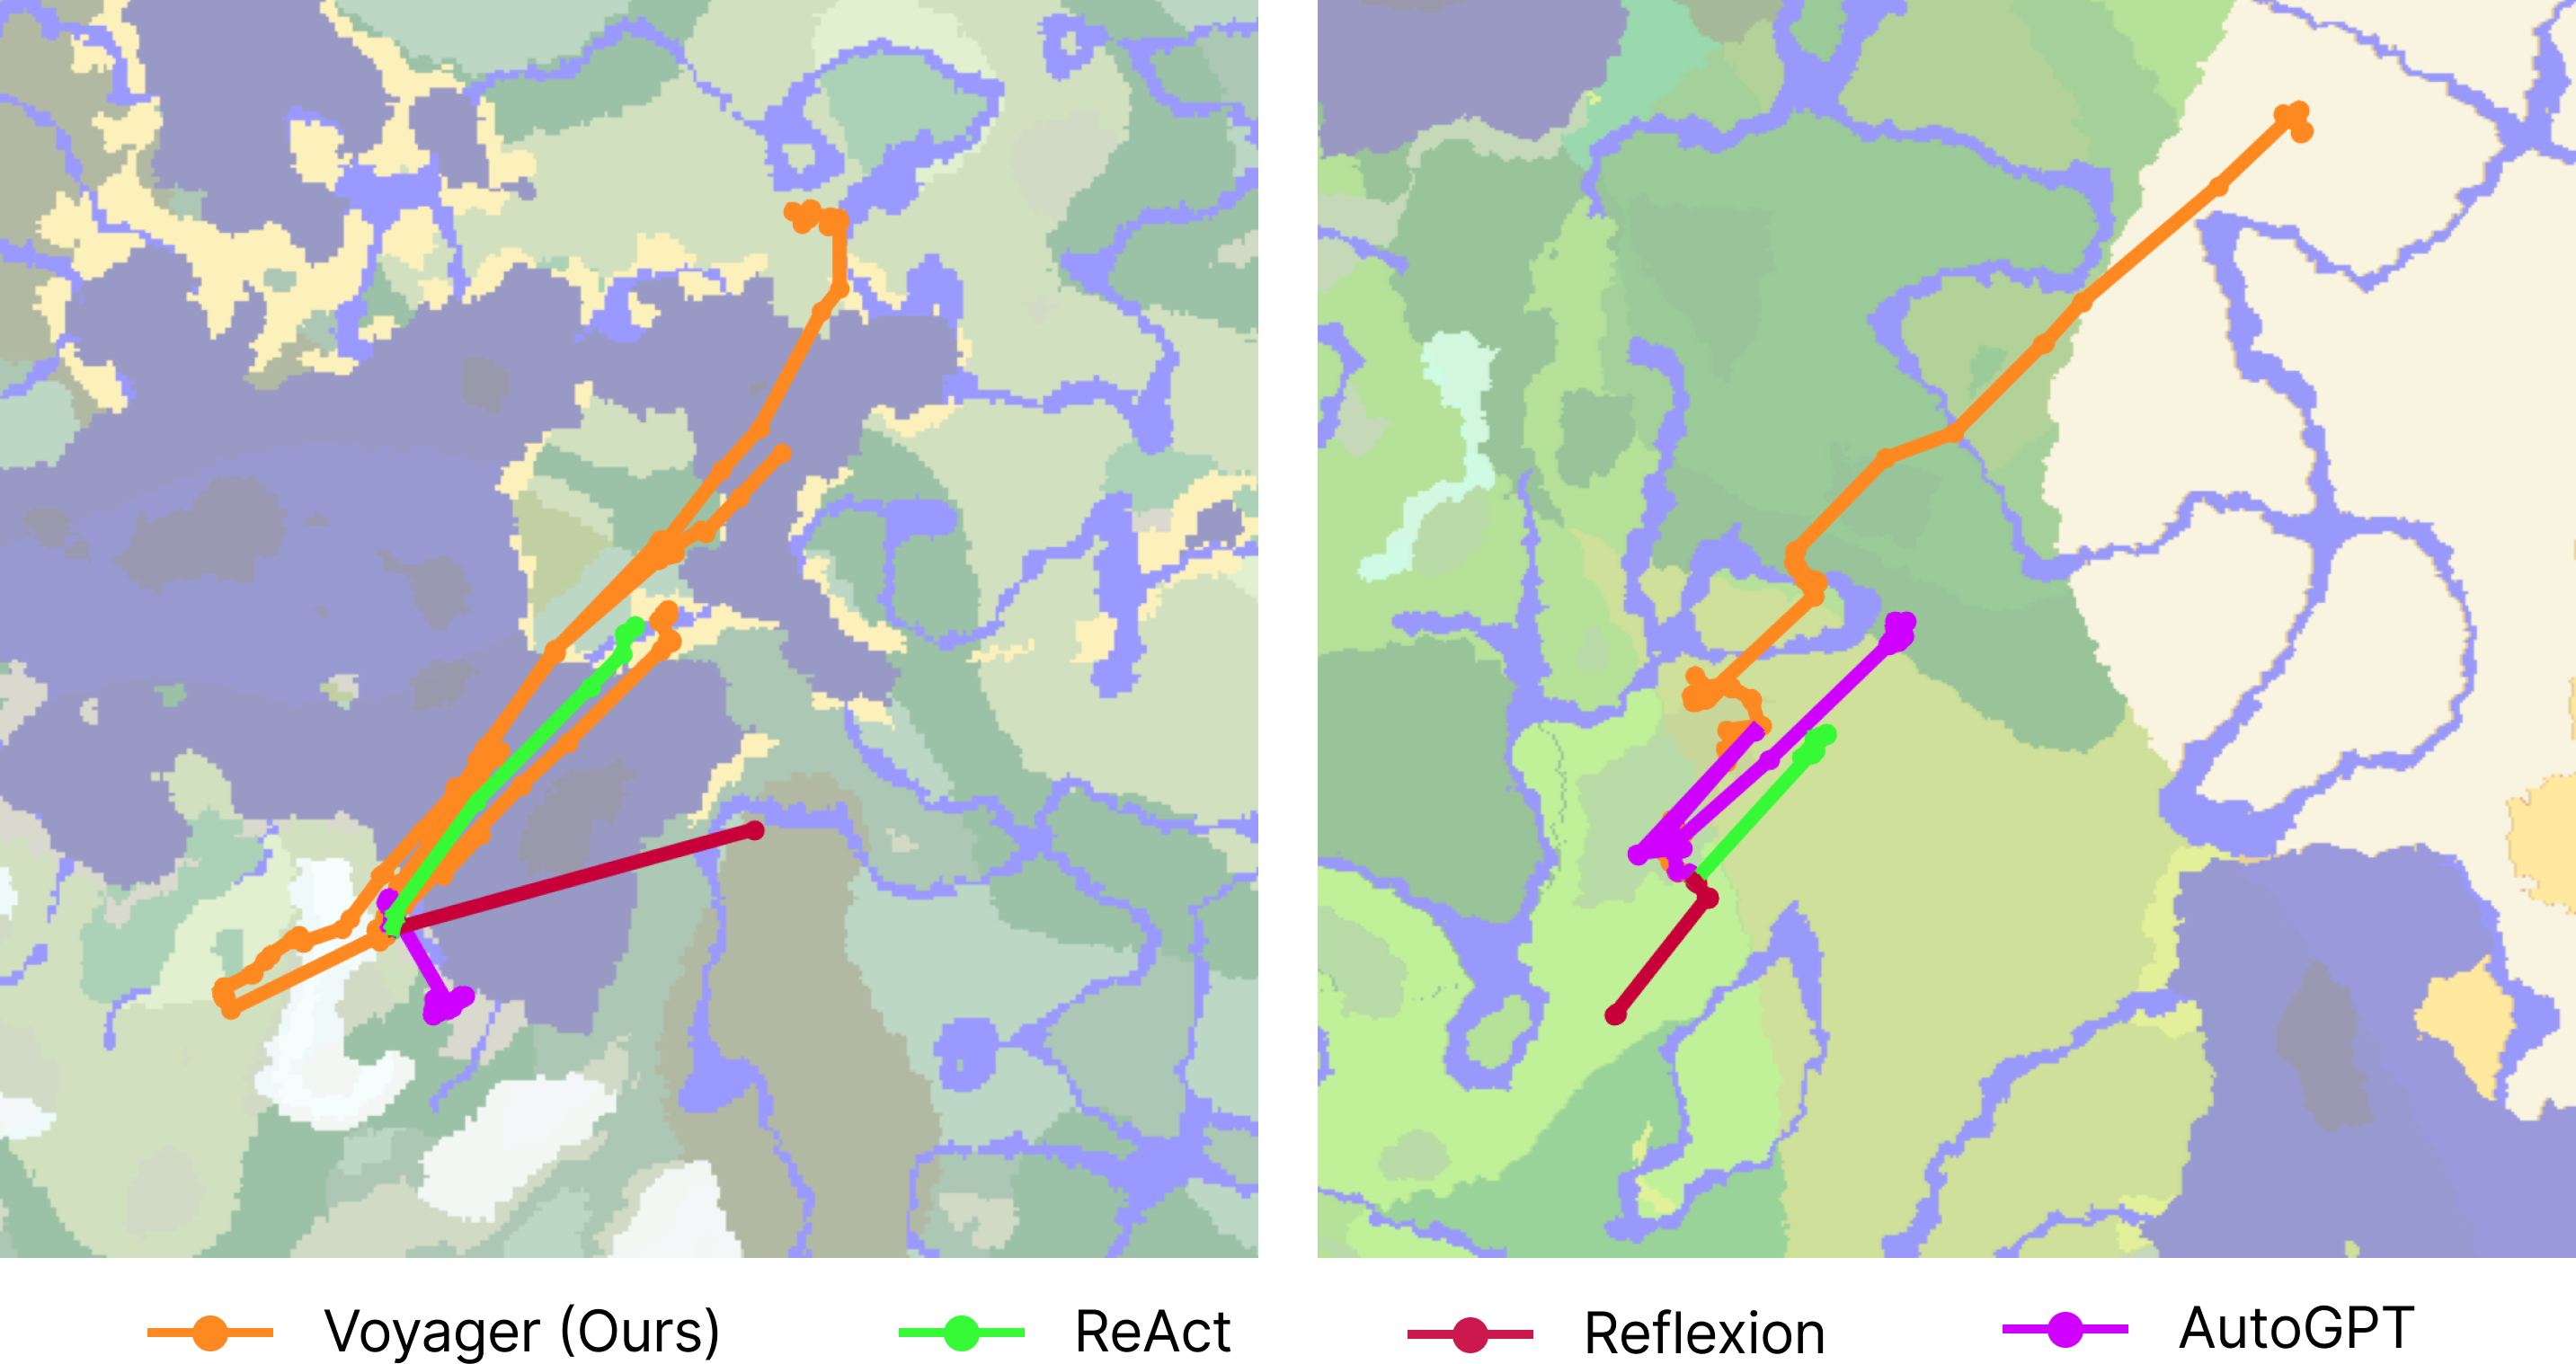
\includegraphics[width=\textwidth]{appendix/figures/map_traj_fig.png}
    \vspace{0.05em}
    \caption{Map coverage: Two bird's eye views of Minecraft maps. \voyager is able to traverse $2.3 \times$ longer distances compared to baselines while crossing diverse terrains. Trajectories are plotted based on the positions where each agent interacts with GPT-4.}
    \label{supp:fig:map}
    \vspace{-1em}
\end{figure}

Agent trajectories for map coverage are displayed in Fig.~\ref{supp:fig:map}. Fig.~\ref{fig:map} is plotted based on Fig.~\ref{supp:fig:map} by drawing the smallest circle enclosing each trajectory.
The terrains traversed by \voyager in each trial is \begin{itemize}
    \item \textbf{Trial 1}: {`meadow', `desert', `river', `savanna', `forest', `plains', `bamboo\_jungle', `dripstone\_caves'};
    \item \textbf{Trial 2}: {`snowy\_plains', `frozen\_river', `dripstone\_caves', `snowy\_taiga', `beach'};
    \item \textbf{Trial 3}: `flower\_forest', `meadow', `old\_growth\_birch\_forest', `snowy\_slopes', `frozen\_peaks', `forest', `river', `beach', `ocean', `sunflower\_plains', `plains', `stony\_shore'.
\end{itemize}
The terrains traversed by ReAct~\cite{yao2022react} in each trial is \begin{itemize}
    \item \textbf{Trial 1}: {`plains', `desert', `jungle'};
    \item \textbf{Trial 2}: {`snowy\_plains', `snowy\_taiga', `snowy\_slopes'};
    \item \textbf{Trial 3}: {`dark\_forest', `dripstone\_caves', `grove', `jagged\_peaks'}.
\end{itemize}
The terrains traversed by Reflexion~\cite{shinn2023reflexion} in each trial is \begin{itemize}
    \item \textbf{Trial 1}: {`plains', `flower\_forest'};
    \item \textbf{Trial 2}: {`snowy\_taiga'};
    \item \textbf{Trial 3}: {`old\_growth\_birch\_forest', `river', `ocean', `beach', `plains'}.
\end{itemize}
The terrains traversed by AutoGPT~\cite{autogpt} in each trial is \begin{itemize}
    \item \textbf{Trial 1}: {`plains', `dripstone\_caves', `savanna', `meadow'};
    \item \textbf{Trial 2}: {`snowy\_taiga'};
    \item \textbf{Trial 3}: {`plains', `stony\_shore', `forest', `ocean'}.
\end{itemize}

\subsubsection{Efficient Zero-Shot Generalization to Unseen Tasks}
\begin{figure}[t]
    \centering
    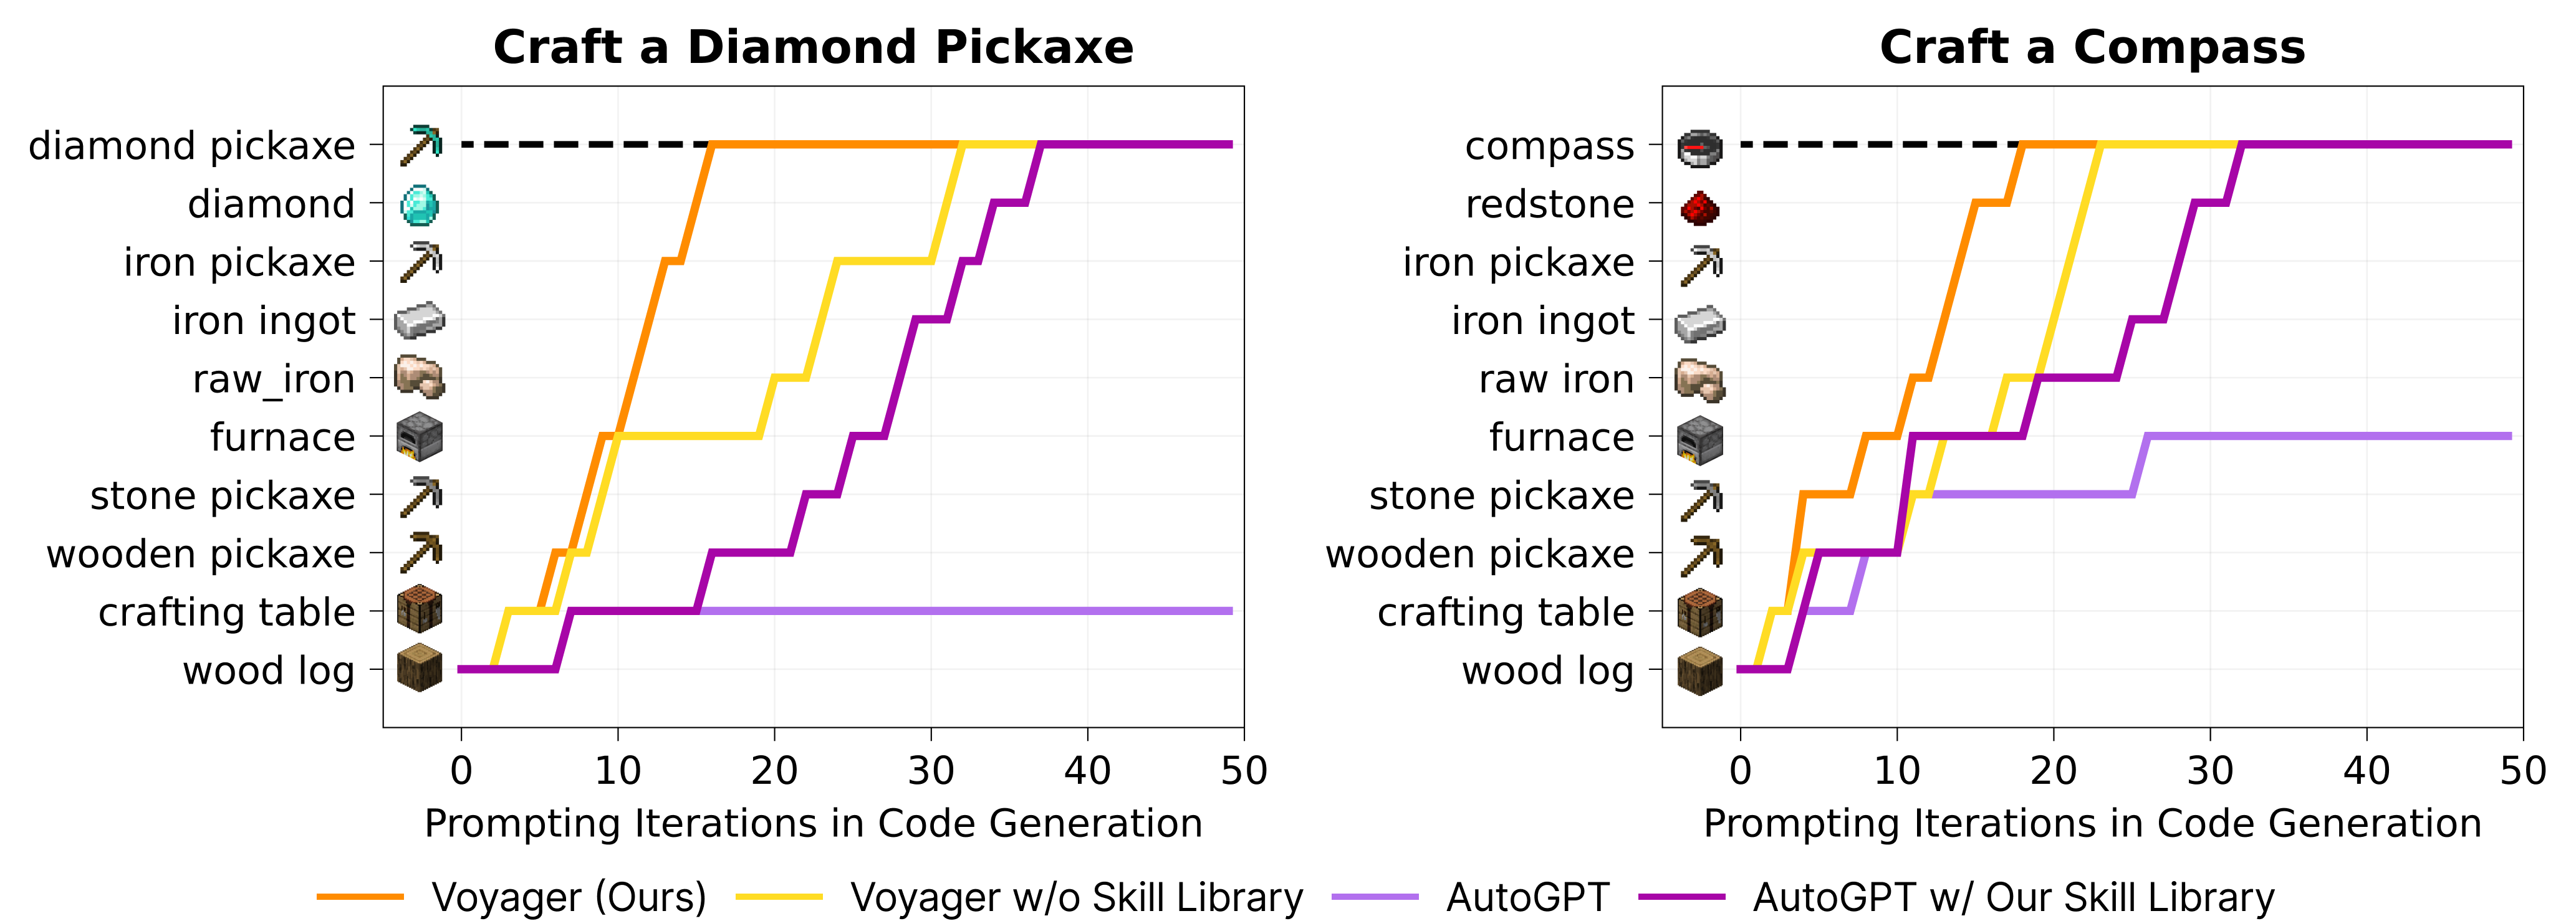
\includegraphics[width=1.0\textwidth]{appendix/figures/downstream_other_fig.png}
    \caption{Zero-shot generalization to unseen tasks. We visualize the intermediate progress of each method on the other two tasks. We do not plot ReAct and Reflexion since they do not make any meaningful progress.}
    \label{supp:fig:downstream}
    % \vspace{-1em}
\end{figure}
\label{supp:sec:zero_shot}
The results of zero-shot generalization to unseen tasks for the other two tasks are presented in Fig.~\ref{supp:fig:downstream}. Similar to Fig.~\ref{fig:downstream}, \voyager consistently solves all tasks, while the baselines are unable to solve any task within 50 prompting iterations. Our skill library, constructed from lifelong learning, not only enhances \voyager's performance but also provides a boost to AutoGPT~\cite{autogpt}.

\subsubsection{Accurate Skill Retrieval}
We conduct an evaluation of our skill retrieval (309 samples in total) and the results are in Table.~\ref{supp:table:skill_retrieval}. The top-5 accuracy standing at 96.5\% suggests our retrieval process is reliable (note that we include the top-5 relevant skills in the prompt for synthesizing a new skill).
\begin{table}[!ht]
\vskip 0.1in
\centering
\caption{Skill retrieval accuracy.}
    \begin{tabular}{ccccc}
        \toprule
        Top-1 Acc & Top-2 Acc & Top-3 Acc & Top-4 Acc & Top-5 Acc \\
        \midrule
        $80.2 \pm 3.0$ & $89.3 \pm 1.8$ & $93.2 \pm 0.7$ & $95.2 \pm 1.8$ & $96.5 \pm 0.3$ \\
        \bottomrule
    \end{tabular}
% \vspace{-1em}
% \vskip -0.1in
\label{supp:table:skill_retrieval}
\end{table}



\subsubsection{Robust to Model Variations}
In the main paper, all of Voyager's experiments are conducted with \texttt{gpt-4-0314}. We additionally run new experiments with \texttt{gpt-4-0613} and find that the performance is roughly the same (Fig.~\ref{supp:fig:model_variations}). It demonstrates that Voyager is robust to model variations. 
\begin{figure}[!h]
    \centering
    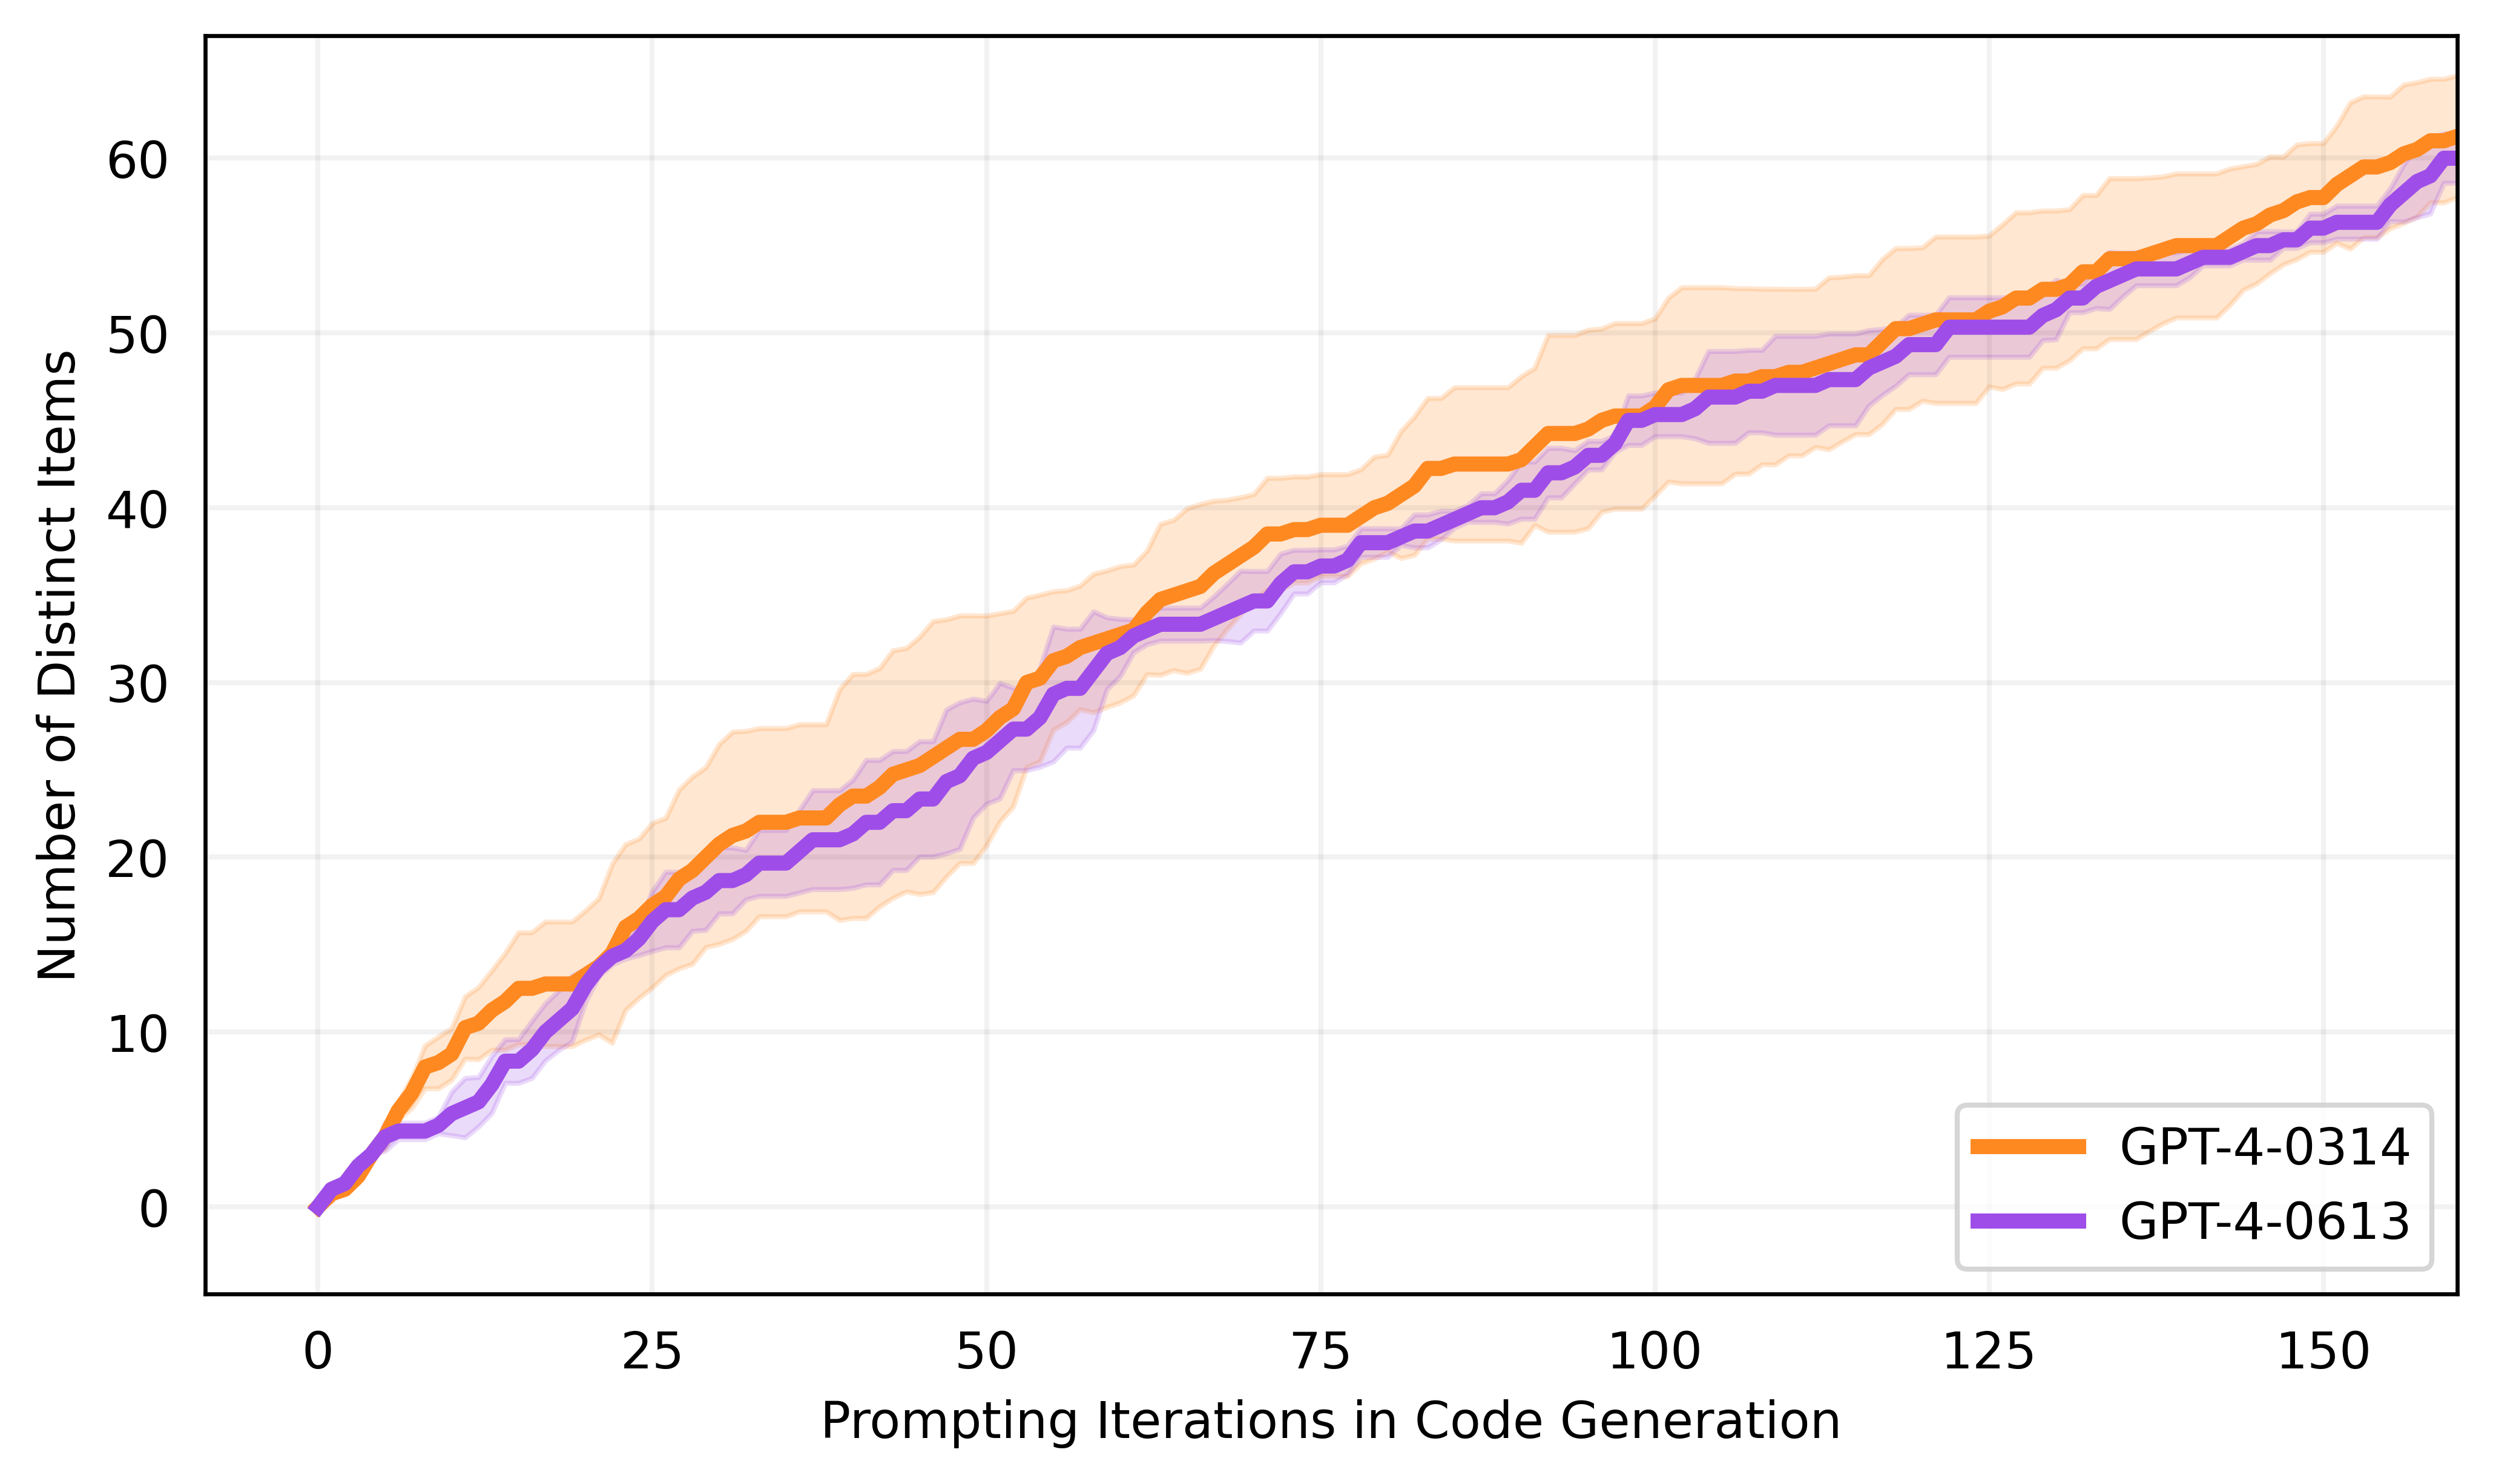
\includegraphics[width=0.7\textwidth]{appendix/figures/model_variations.png}
    \caption{\voyager's performance with GPT-4-0314 and GPT-4-0613.}
    \label{supp:fig:model_variations}
\end{figure}
% \subsubsection{Examples of Execution Traces}
% Examples of execution traces among the curriculum agent (for automatic curriculum), the action agent (for code generation), the critic agent (for self-verification), and the skill manager (for adding new skills and skill retrieval) are included in the supplementary folder. 